\documentclass{article}
\usepackage[english]{babel}
\usepackage{graphicx}
\usepackage{graphicx,scalerel}
\begin{document}

\section*{Task 2:}

\subsection*{2a)}

mean = 33.55274553571429 \newline
standard deviation  = 78.87550070784701

\subsection*{2b)}
See code for implementation.
\subsection*{2c)}

\begin{figure}[h!]
    \centering
    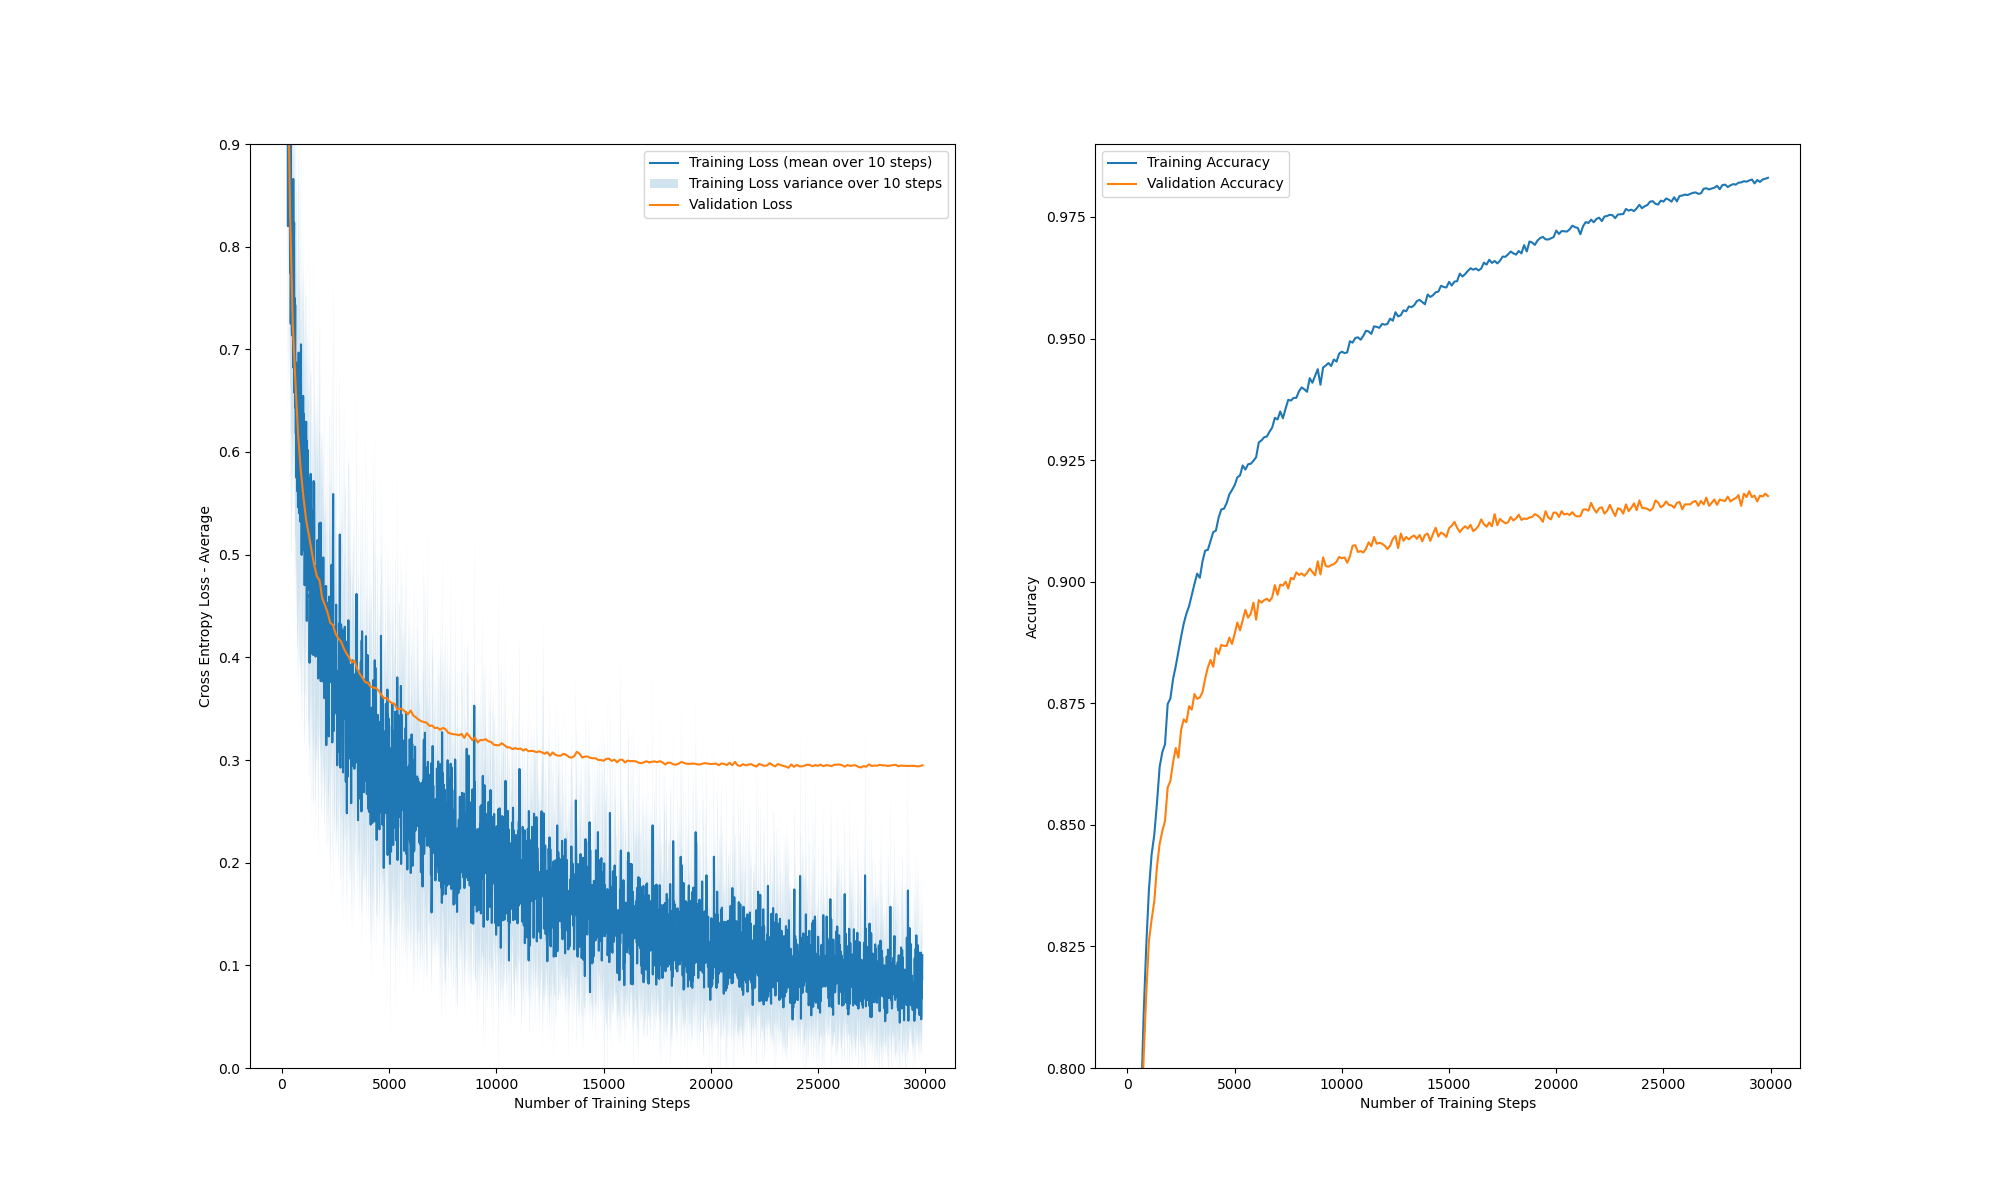
\includegraphics[width=\linewidth]{task2c_train_loss.png}
    \caption[short]{Plot of the training and validation loss and accuracy over training. We can clearly see sign of overfitting from the plot. }
\end{figure}


\subsection*{2d)}

We have an input layer with the size of 784. In addition we have 1 bias unit. The hidden layer will
get input from 785 nodes. Further, it has 64 nodes, which means there are 64 weights. We will 
get 785 * 64 parameters in this layer. In the next layer we have 10 nodes and it gets input from 64 nodes. This 64 *10 parameters.
In total we will have : \newline
\begin{equation}
    Number of parameters = 785 \cdot 64 + 64 \cdot 10 = 50880 
\end{equation}


\section*{Task 3 :}
\subsection*{3a)}
See code for implementation.
\subsection*{3b)}
See code for implementation.
\subsection*{3c)}
See code for implementation.
\newline

Generally, the model converge faster and we are getting higher accuracy when we are using the improvments from task 3a, task 3b and task 3c.
From the figure we can see that when improved weights  are implemented, the model achieve a much higher accuracy compared to the model form task 2. However we
can see that the model do not converge much faster compared to the model from task 2. 

Further, improved sigmoid have been implemented.  The model with improved sigmoid converge much faster. From the figure we can see that the early stopping kicks inn for approximately 13000 steps.
The result make sense since we know improved sigmoid has a steeper gradient near its origin , which allows for faster convergence. This means
the weights in the network can be updated more quickly, leading to faster training times. 
In addition, we can see that the accuarcy of the system improved. 

Lastly, by using momentum , the model achieves early stopping at approximately 10000 steps. There is not much different in accuarcy compared to the model with improved sigmoid and improved weights. 
While momentum can be useful in accelerating convergence and improving optimization in deep neural networks with many layers, it may not be as beneficial or can even be harmful in shallow neural networks with only a few hidden layers. 
This is because in shallow neural networks, the weight space is generally less complex, and momentum may cause the optimizer to overshoot and oscillate around the optimal weights, resulting in slower convergence or even worse performance.




\section*{Task 4 : }

\subsection*{4a)}

The figure shows the model's performance with hidden units to 32.
Compared to the figure from task 3, we observe that the validation accuracy is much lower. In addition, we can see the model with momentum performs have decreased compared to 
the figure from task 3. This change in performance make sense since the weight is less compelx with 32 hidden units in hidden layer. 

\subsection*{4b)}

The shows the model's performance with 128 units in hidden layer. Compared to the figure from task 3,  we observe that the validation accuracy is much higher.
In addition, we can see that the model with momentum performs much better. This is because the weight space is more compelx now compared to taks 3 and task 4b. 


\subsection*{4c)}

In task 3 we have had 508080

\subsection*{4d)}
    
\subsection*{4e)}

\subsection*{4f)}


\end{document}